\renewcommand{\arraystretch}{1.5}
\chapter[Jake \LILLYxBOXxVersion{\small 1.0.8}]{Jake}
\elable{mrk:JAKE}\TitleSUB{\Jake[]! Would you get me the cake please?\ldots \hfill \LILLYxBOXxVersion{\small 1.0.8}}
\section{Grundlegendes}\elable{jmp:iJake}
\subsection{Entwicklung}
Anfänglich wurde \Jake als \emph{installer} konzipiert, der einfach nur die mühsehlige Installation
des Pakets abnehmen soll. Mittlerweile hat sich \Jake allerdings weiterentwickelt und
bietet das Potenzial für einiges mehr. Im Folgenden sei die Funktionsweise genauer erklärt.
Zu beachten ist allerdings, dass \Jake bisher nur für Linux und MacOS einen Installer und somit
seine Funktionalität zur Verfügung stellt!

\subsection{Die Installation}
\elable{mrk:InstallJake}Jake wird als \T{.jar}-Datei geliefert und lässt sich, eine vorhandene Installation von Java vorrausgesetzt, durch das bloße ausführen installieren. Auf Linux kann dies zum Beispiel wie folgt von statten gehen:
\begin{bash*}
java -jar jake.jar
\end{bash*}
Nach abgeschlossener Installation sollte das Terminal neu gestartet, oder die Konfigurationsdatei neu geladen werden, um Jake zur Verfüung zu stellen. Das bloße Ausführen von \cbash{jake} sollte nun eine Hilfe anzeigen, die über die jeweiligen Optionen aufklärt.

\begin{bemerkung}[C++ Jake]
\textit{Bis zur Version \LILLYxBOXxVersion{1.0.9} war Jake in C++ geschrieben jund benötigt deswegen eine andere Installation.}\newline
\Jake zu installieren sollte normalerweise einem Kinderspiel gleichen. Notwendig sind hierfür
auf allen bisher unterstützten Betriebssystemen (Debian-Basiertes Linux und MacOS) ein
\verb|C++14| fähiger \T{gcc}-Compiler und \T{make}.
Anschließend gilt es ins \verb|jake_source|-Verzeichnis zu navigieren.
Es befindet sich hier: \T{Lilly/Jake/jake\_source}.
In diesem Verzeichnis kann man nun \T{make} ausführen. Dies sorgt dafür,
dass nicht nur \T{jake.cpp} zu einer ausführbaren Datei wird, sondern auch,
dass \LJake systemweit zur Verfügung steht (sofern die verwendeten Konsole
bash, zsh oder iTerm ist, bzw. im allgemeinen auf eine der folgenden Dateien
zugreift: \T{.bashrc}, \T{.zshrc}, \T{.bash\_profile}).\newline
Damit gilt \Jake als \emph{installiert}.
\end{bemerkung}


\subsection{Lilly mit Jake installieren}
Mit \LILLYxBOXxVersion{2.0.0} liefert \Jake stets eine Version von Lilly mit, die sich nach einem Update automatisch mit dem nächsten Start von \Jake aktualisiert, sofern sie einmal installiert wurde: \bbash{jake install}. Wird hier eine Frage nach verschiedenen Installationsoptionen gestellt, so siehe bei den \jmark[Entwicklerinformationen]{mrk:jakedevinfo} oder wähle einfach die Intallation der enthaltenen Variante (vermutlich Option $2$). Die automatische Aktualisierung wird durch eine Ausgabe getreu \T{[Die Lilly-Installation wurde aktualisiert.]} ausgegeben. Mithilfe von \bbash{jake GUI} kann Jake auch über die Kommandozeile im Grafischen-Modus gestartet werden, allerdings empfiehlt sich hierfür das Verwenden des Eintrags im Anwendungsmenü.

\subsection{Jake im Überblick}
Hier werden zuerst die Vorzüge der Kommandozeile präsentiert, da die grafische Variante von Jake noch nicht sinnvoll ausgebaut ist und sich bisher lediglich zum editieren von Konfigurationsdateien eignet.
\paragraph{Kommandoszeile}
\elable{mrk:jakesettings}Im Regelfall, zur Kompilierung eines Dokuments, genügt es \Jake mit dem jeweiligen Dokument aufzurufen:
\begin{bash*}
jake :lan:Dokumentname.tex:ran:
\end{bash*}
Der Kompilierung können nun eine endlose Reihe an Einstellungen übergeben werden die jeweils mit einem \say{\T{-}} anzuführen sind. Eine boolesche Einstellung kann so bereits umgeschaltet werden. So liefert:
\begin{bash*}
jake dump -debug -debug -debug
\end{bash*}
Für die Einstellung \say{\T{debug}} \emph{true}. Eine \say{normale} Einstellung, welche ein Argument fordert wird durch einen Doppelpunkt beendet:
\begin{bash*}
jake dump -lilly-author: "Sonnenprophet Hamsterbacke"
\end{bash*}
Liefert den entsprechenden Author für \T{lilly-author}. Dies lässt sich auch bei booleschen Ausdrücken, hier mit dem Setzen der Werte \emph{true} und \emph{false} erzeugen. Final gibt es noch Listen, die auch so zugewiesen werden können, allerdings durch das anfügen von \T{+:} auch erweitert werden können. So liefert:
\begin{bash*}
jake dump -lilly-boxes: "DEFAULT" -lilly-boxes+: "ALTERNATE"
\end{bash*}
Den Wert \say{\T{DEFAULT ALTERNATE}} für die Einstellung \T{lilly-boxes}, die Trennung der Elemente (Leerfeld) wird von Jake automatisch erkannt ist aber in der Regel auf Leerfelder normiert.\\
Hier die große (und hoffentlich vollständige) Liste aller möglichen Einstellungen. Ist der Standardwert zu lang, so wird er durch \T{\ldots} gekürzt, wenn er abhängig ist, wird dies in der Bemerkung erklärt. Es gilt zu beachten, dass sich durch Konfigurationsdateien alle Einstellungen modifizieren lassen und somit auch die Standardwerte verändern:{%\renewcommand{\arraystretch}{0.95}
\begin{tabularx}{\linewidth}{t~i~t~^>{\scriptsize}m{0.3\linewidth}+}
    \toprule
        \headerrow Bezeichner & Typ & Defaultwert & \normalsize Beschreibung \\
    \midrule
        Version & String & [\ldots] & Aktuelle Version von Jake \\
        \headerrow* file & String & dummy.tex & Datei, um die es gehen soll \\
        answer & String & & Antwort, die, sofern nicht leer, auf alle Fragen die Jake stellt zuerst gegeben wird. Ein setzen auf \say{\T{y}} entspricht der \T{-y}-Option von \T{apt}.\\
        \headerrow* operation & String & help & Was Jake tun soll \\
        debug & Boolean & false & Gibt an, ob Debug ausgegeben werden soll oder nicht \\
        debug-filter & String & .* & Veraltet \\
        path & String & ./ & Pfad zu Lilly \\
        what & String & & Zusatzargument für manche Operationen \\
        install-path & String & \${HOME}/texmf & Ziel Pfad der Installation \\
        gepardrule-path & String & & Pfade für Gepardregeln (durch \say{\T{:}} getrennt)\\
        autoconf & Boolean & true & Soll automatisch eine \T{.conf}-Datei gewählt werden? \\
        comment-pattern & String & ![\char`\^!]*! & Kommentarmuster \\
    \midrule
        lilly-path & String & \$(dirname\ldots & Pfad zur \T{Lilly.cls} \\
        lilly-out & String & ./\$(BASE\ldots & Ausgabeordner der Tex-Datei? \\
        lilly-in & String & ./ & Input-Pfad für Dateien \\
        lilly-nameprefix & String & & Namenspräfix für Ausgabedatei \\
        lilly-boxes & List & DEFAULT & Boxen für den Kompiliervorgang \\
        lily-modes & String & default & Modi für den Kompiliervorgang \\
        lilly-complete & Boolean & true & Vollständige Dokumentvariante \\
        lilly-complete-name & String & COMPLETE- & Präfix der vollständigen Version \\
        lilly-print-name & String & PRINT- & Präfix der Druckversion \\
        lilly-cleans & List & log aux \ldots & Dateiendungen die von \T{autoclean} gelöscht werden \\
        lilly-autoclean & Boolean & true & Sollen Dateien automatisch gelöscht werden? \\
        lilly-compiletimes & String & 2 & Wie oft soll kompiliert werden \\
        lilly-vorlesung & String & NONE & Um welche Vorlesung handelt es sich? \\
        lilly-semester & String & 0 & Das wievielte Semester ist es \\
        lilly-n & String & 42 & Um das wievielte Übungsblatt handelt es sich? \\
        lilly-show-boxname & Boolean & true & Soll der Boxname angezeigt werden? \\
        lilly-layout-loader & String & & Pfad zu den Layouts \\
        lilly-external & Boolean & false & Soll versucht werden, Grafiken auszulagern? \\
        lilly-external-out & String & extimg & Ausgabeordner für ausgelagert Grafiken \\
        \headerrow* lilly-author & String & Florian\ldots & Author des Dokuments \\
        \headerrow* lilly-author-mail & String & florian.s\ldots & Email-Adresse des Authors \\
        lilly-signatur-farbe & String & Leaf & Farbe für das Highlighting \\
        lilly-bibtex & String & & Bibtex-Datei (ohne Endung) \\
        lilly-doctype & String & Mitschrieb & Typ des Dokuments \\
        lilly-configs-path & String & & Pfad zur Lilly-Konfigurationsdatei (\blankcmd{lillyPathConfig})\\
        lilly-data-path & String & & Pfad zu generellen Daten (\blankcmd{lillyPathData})\\
        \midrule
        jobcount & String & 2 & Wie viele verschiedene Threads sollen im multithreaded-compile gleichzeitig betrieben weren? \\
        error-count & String & 5 & Wie viele Fehler sollen in der Vorschau maximal angezeigt werden? \\
        mk-name & String & Makefile & Veraltet, Name des Makefiles \\
        mk-path & String & ./ & Veraltet, Pfad des Makefiles \\
        mk-use & Boolean & false & Veraltet, soll das Makefile verwendet werden? \\
    \bottomrule
\end{tabularx}
}
Zusätzlich kann anstelle der vorangestellten Option wie \T{dump} beziehungsweise der \T{.tex}-Datei auch eine Konfigurationsdatei angegeben werden. Auf sie wird \jmark[hier]{mrk:configfile} % todo: link
mehr eingegangen. Bei einer solchen Angabe handelt es sich um eine Kurzform der jeweiligen Optionen \T{config} und \T{file\_compile}. Ausführlich würde man also zum Kompilieren dieser Dokumentation schreiben:
\begin{bash*}
jake file_compile -file: Lilly-Dokumentation.doc.tex
\end{bash*}
beziehungsweise, zum Verwenden der beiliegenden Konfigurationsdatei:
\begin{bash*}
jake config -file: doc.conf
\end{bash*}
Oder eben die Kurzform:
\begin{bash*}
jake doc.conf
\end{bash*}
Die automatisch die Optionen entsprechend setzt.\smallskip\newline
Als letzte wichtige Funktion sei noch \T{get} genannt, welche für das Paket \LILLYxNOTExLibrary{LILLYxGRAPHICSxPROVIDER} aus \LILLYxNOTExLibrary{LILLYxGRAPHICS} relevant ist. So liefert der Befehl:
\begin{bash*}
jake get
\end{bash*}
Eine PDF wie die folgende, die alle mit Lilly gelieferten Grafiken enthält:
\begin{tcbraster}[raster columns=3, blankest, graphics pages={13,33,34},colback=white]
    \tcbincludepdf{\LILLYxPATHxDATA/Graphics/all-OUT/all.pdf}
\end{tcbraster}
Angezeigt wurden hier übrigens die Seiten $13$, $33$ und $34$ zum Kompilierzeitpunkt dieser Dokumentation.
\paragraph{Gui}
Wie bereits angemerkt, ist die GUI von \Jake noch nicht ansatzweise ausgereift. Der sich öffnende Hauptdialog erlaubt das Auswählen einer Latex- oder Konfigurationsdatei und zeigt die aus der Datei extrahierten Informationen inklusiver ihrer (sofern verschieden) extrahierten Werte an:
\begin{center}
    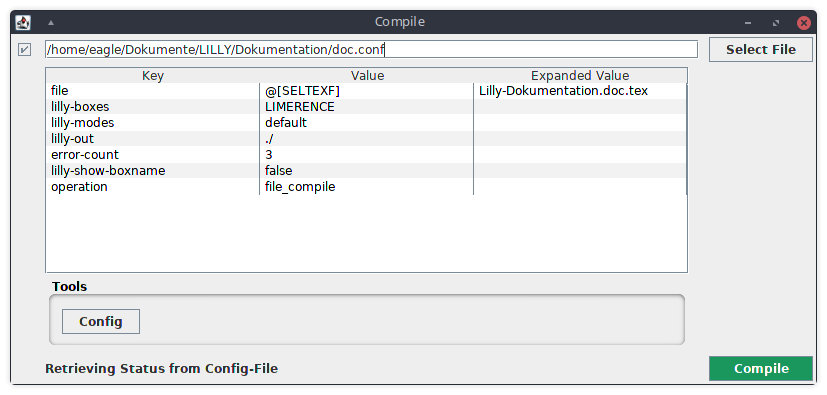
\includegraphics[width=0.75\linewidth]{Data/Bilder/JakeGUIMain.png}
\end{center}
Nebst einem schönen Ausblick auf das was in der GUI-Welt noch so alles geschehen mag, bietet sich der Button \T{Config} an, der im Falle keine ausgewählten Konfigurationsdatei einfach auf einer neuen arbeitet:
\begin{center}
    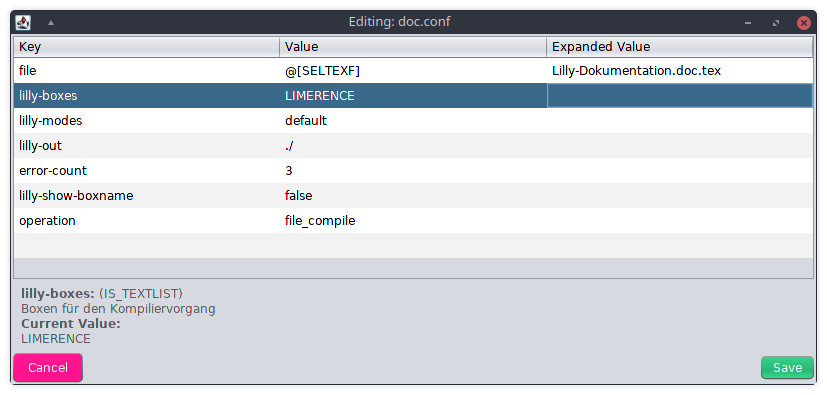
\includegraphics[width=0.5\linewidth]{Data/Bilder/JakeGUIConfig.png}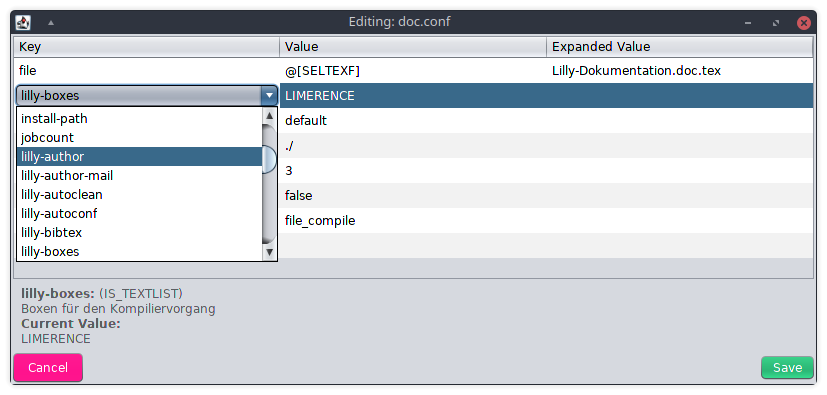
\includegraphics[width=0.5\linewidth]{Data/Bilder/JakeGUIConfigSelection.png}
\end{center}
Hier werden nicht nur einige Informationen zu den jeweileigen Einstellungen angezeigt, sondern auch Plausibilitätsprüfungen durchgeführt. Im Falle einer neuen Konfigurationsdatei kann beim Speichern ein entsprechendes Ziel ausgewählt werden.

\subsection{Entwicklerinformationen}
\elable{mrk:jakedevinfo}% Note that update will occur even if lilly hasn't updated, but jake has.
Wenn du an \Jake oder Lilly mitentwickelst, oder einfach generell immer die aktuellste Version von Jake haben möchtest, so gilt es ein paar Schritte zu befolgen. Vorab: \Jake wurde als Maven-Projekt angelegt, zum generieren der neusten Version ist also Maven für die jeweilige Plattform vonnöten (Beispiel: \cbash{sudo apt install maven})
\begin{enumerate}\narrowitems
    \item Klone das Git-Repository (\url{https://github.com/EagleoutIce/LILLY})
    \item Navigiere in das Verzeichnis \T{Jake/} im Repository
    \item Generiere die neuste \Jake-Version: \begin{bash*}
mvn clean install
        \end{bash*}
    \item Wähle aus (beachte die Angabe einer \jmark[Nutzerkonfiguration]{mrk:jdefconf}): \begin{description}
        \item[stable] Diese Installation wird unregelmäßig aktualisiert und entspricht der \T{jake.jar}, muss also nicht extra gebaut werden. Diese Variante empfiehlt sich für Tests und für die Entwicklung an Lilly, da so Fehler auf Seiten von \Jake in der Regel ausgeschlossen werden können.
        \item[rolling] Diese Installation wird nicht über das \T{git}-Repository synchronisiert sondern kann vom Nutzer bei Bedarf erzeugt werden. Hierzu einfach im \T{Jake}-Verzeichnis, den obigen Befehl (\bbash{mvn clean install}) ausführen. Im Unterverzeichnis \T{target/} befinden sich danach die \T{development-jake.jar}, die nach dem Ausführen mit jedem weiteren Kompilieren von \Jake automatisch aktualisiert: \begin{bash*}
java -jar development-jake.jar
        \end{bash*}
    \end{description}
    \item Bei der Installation von Lilly mit \bbash{jake install}\footnote{Nicht vergessen, dass Terminal neu zu starten/die Konfigurationsdatei der Konsole neu einzulesen.} wird nun sicher eine Frage erscheinen, welche Variante von Lilly installiert werden soll. Während im \T{stable}-tree beide Optionen theoretisch verwendbar sind, so empfiehlt sich - auch um immer die aktuellste Lilly-Version zu haben, die Verlinkung der gefunden Lilly-Instanz. Hier allerdings Vorsicht, da der Pfad zur \T{Lilly.cls} falsch sein kann. Der Pfad sollte in seiner Signatur auf \T{LILLY/Lilly/Lilly.cls} enden. Ist dies nicht der Fall, so muss die Option \T{lilly-path} angegeben werden, die den (am besten absoluten) Pfad zur \T{Lilly.cls} angibt.
\end{enumerate}

\section{Gepard}
\elable{mrk:Gepard}Die \textbf{Ge}nerator-\textbf{Par}ser-\textbf{D}escriptor-Language ist die Sprache, in der alle Konfigurationen und Erweiterungen von Jake formuliert sind. Im Kern des Parsen von Dokumenten steht der \T{Tokenzier} der erlaubte Zeichen und Zuweisungen unterscheidet, und vom \T{Configurator} erweitert wird. Dieses Konfigurationsmodul gestattet die Definition von \jmark[Konfigruationsdateien]{mrk:configfile}, die durch einfache Zuweisungen die Einstellungen von \Jake kontrollieren können. Darüber baut das namensgebende Gepard-Modul auf, welches verschiedene Boxen und damit verschiedene Erweiterungen gewährt, wobei bisher ein verschachteln dieser Boxen nicht vorgesehen ist. Die einzelnen Module werden weiter \jmark[unten]{gpd:modules} beschrieben.
\begin{bemerkung}[Kommentare]
    Ein Kommentar in Gepard wird in der Regel durch Ausrufezeichen markiert. Sollten diese allerdings verwendet werden müssen, so ist es möglich die Sequenz für Kommentare mithilfe von \T{comment-pattern} zu modifizieren:
\begin{gepard}
debug   = true
! debug = false !
what    = /* Noch kein Kommentar */
comment-pattern = /\*.*\*/
lilly-author    = Hallo !*! Sonne !*!
answer  = 42, !*\lstcomment{/*~Ich bin jetzt ein Kommentar :D */}*!
\end{gepard}
Wir erhalten (mit \T{dump}) die Ausgabe für die modifizierten Werte:
\begin{bash*}
comment-pattern     :  [/\:star:.:star:\:star:/]
debug               :  [true]
lilly-author        :  [Hallo ! Sonne !]
what                :  [/:star: Noch kein Kommentar :star:/]
answer              :  [42,]
\end{bash*}
Keine mit Jake gelieferte Konfigurations- oder anderweitige Datei modifiziert die Syntax für einen Kommentar.
\end{bemerkung}

\subsection{Konfigurationsdateien}
\elable{mrk:configfile}Eine Konfigurationsdatei endet für gewöhnlich auf \T{.conf}, wobei diese Endung lediglich von der Autovervollständigung und der GUI anerkannt wird, allerdings keineswegs verpflichtend ist, \Jake versucht jede Konfigurationsdatei entsprechend zu parsen. Erlaubt werden alle auch für \Jake in der Kommandozeile verwendbaren \jmark[Einstellungen]{mrk:jakesettings}, wobei zur Zuweisung hier \T{=} und \T{+=} anstelle von \T{:} und \T{+:} verwendet werde und kein \say{\T{-}} angeführt wird. So kann eine Konfigurationsdatei wie folgt aussehen:
\begin{gepard}
operation           = file_compile
file                = @[SELTEXF]
lilly-modes         = default
lilly-show-boxname  = false
lilly-boxes        += LIMERENCE
lilly-out           = ./
error-count         = 3
\end{gepard}
Auch wenn hier zur Optik die Zuweisungen alle auf die gleiche Einrückung gesetzt wurden, so ist dies nicht zwinged und auch Tabs und Leerfelder haben im Verhältnis zur Zuweisung keine semantische Bedeutung und sind auch syntaktisch irrelevant. Das hier enthaltene \T{@[SELTEXF]} ist ein \jmark[Expandable]{gpd:expandables}, welches über ein weiteres Gepard-Modul definiert wird. Dieses evaluiert zur ersten TeX-Datei die im Ordner gefunden wird, hat also den Vorteil, dass diese Einstellung der konfigurationsdatei nicht immer wieder angepasst werden muss. Es gibt einige derartige Einstellungen.
\begin{bemerkung}[Setzen von \T{operation}]
    Es ist zwangsläufig zu empfehlen die Einstellung \T{operation} auf das gewünschte Ziel zu überschreiben, da sonst die neue Datei (sofern überhaupt eine andere angegeben wurde) wieder mit der \T{config}-Opteration ausgeführt wird, was im Zweifelsfall zu einer Endlosrekursion führen kann (diese wird von \Jake natürlich erkannt und abgebrochen).
\end{bemerkung}
Weiter besitzt \Jake die \jmark[Einstellung]{mrk:jakesettings} \T{autoconf}, die eine Konfigurationsdatei bei der Wahl einer TeX-Datei auch automatisch auswählen kann sofern diese den gleichen Namen oder den Namen \T{jake.conf} trägt. So wird zum Beispiel beim Kompilieren von \T{Dokument.tex} automatisch die Datei \T{Dokument.conf} als Konfigurationsdatei geladen, sofern diese existiert. Analog würde die \T{jake.conf} gewählt werden, wenn sie existiert.
\begin{bemerkung}[Standartkonfigurationsdateien]
    \elable{mrk:jdefconf}Jake selbst kommt mit der \T{jake\_default.conf}, das ist eine Konfigurationsdatei, die für den aktuellen Build Einstellungen setzt, ohne jedesmal die in den \T{CoreSettings} vermerkten Einstellungen zu modifizieren. Diese Datei lässt sich theoretisch problemlos anpassen, davon wird allerdings stark abgeraten, da derartige Modifikationen mit einer Aktualisierung von \Jake wieder überschrieben werden. Allerdings kann bei der Installation von \Jake die Einstellung \T{path} gesetzt werden um eine Nutzerkonfiguration anzugeben. Diese wird von da an immer beim Starten von \Jake eingelesen und verarbeitet:
    \begin{bash*}
java -jar jake.jar -path: /pfad/zu/meiner/Konfiguration.conf
    \end{bash*}
    Eine vorhandene Jake-Installation (auch zum Abändern dieses Pfades) kann mithilfe von \cbash{jake DEI} deinstalliert und mit \cbash{jake REI} reinstalliert werden, so kann auch bei einer bestehenden Installation von Jake mithilfe von:
    \begin{bash*}
jake REI -path: /neuer/pfad/zu/meiner/Konfiguration.conf
    \end{bash*}
    Der Pfad aktualisiert und mit:
    \begin{bash*}
jake REI
    \end{bash*}
    Der Nutzerpfad gelöscht werden. So Kann man mit dieser Konfiguration den Author aller Dokumente auf sich verändern:
    \begin{gepard}
! Setze Autor für alle Dokumente: !
lilly-author       = Kalle Uweson
lilly-author-mail  = kalle.uweson@hotmail.waffle
! Verstecke standardmäßig den Boxnamen: !
lilly-show-boxname = false
! Setze standardbox auf ALTERNATE !
lilly-boxes        = ALTERNATE
    \end{gepard}
    Aktuell wird überlegt, ob bei der Instalation direkt nach wichtigen Daten wie dem Namen gefragt wird.
\end{bemerkung}

\subsection{Gepard Module im Allgemeinen}
\elable{gpd:modules}Gepardmodule werden in einer Datei als Box präsentiert. Eine Datei kann so etliche verschiedene Boxen und damit Konfigurationen für verschiedene Module halten und verarbeiten. Das grundlegende Gepard-Modul kann in einer (üblicherweise auf \T{.gpd} endenden) Datei wie folgt dargestellt werden:
\begin{gepard}
BEGIN :lan:modul:ran:
    :lan:Modulspezifikation:ran:
END
\end{gepard}
In die jeweiligen Start- und Endzeilen können beliebige Zeichen zur Übersicht Platziert werden, sie werden verworfen, was zum Beispiel folgende Spezifikation genauso valide macht:
\begin{gepard}
BEGIN :lan:modul:ran::
    :lan:Modulspezifikation:ran:
END;
\end{gepard}
Die Spezifikation besteht in der Regel aus Konfigurationsähnlichen Zuweisungen, die je nach Modul eine unterschiedliche semantische Bedeutung haben. Die gewünschten Konfigruationen können über die Einstellung \T{gepardrule-path} % CHANGE THIS TO A LIST AND FIX IF FILES AREN'T VALID :D
gesetzt werden, wobei die Pfade durch einen \say{\T{:}} getrennt sind. Bisher muss vom Nutzer die Existenz der zugrundeliegendne Dateien gewährleistet werden.

\subsection{Buildrules}
Buildrules definieren den Modus in dem das Dokument kompiliert wird. So definieren sie den \T{print} und den \T{default} Modus. Die Box trägt den Namen \T{buildrule} und muss einen Namen, einen Anzeigenamen und einen Modus definieren. Im Folgenden die Definition des \T{default}-Modus, die Kommentare sollten die Anforderungen zu Genüge erklären:
{\lstfs{7}% Smaller listing
\begin{plaingepard}
BEGIN buildrule: ! Der Doppelpunkt ist optional. Ich mag ihn, man braucht ihn nicht !

    ! Das Einrücken _und_ die Leerfelder sind optional. !
    ! Allerdings sollten erstmal nur Leerfelder verwendet werden !
    ! Mit X sind Zuweisungen markiert die verpflichtend sein sollen (aber nicht sind) !

!X!  name                   = default     ! buildrule name für lilly-modes !

!X!  display-name           = Standard    ! Anzeigename (Standard-Version) !

!X!  lilly-mode             = default     ! Welcher Modus soll an Lilly übergeben werden? !
                                          ! Info: Diese können noch nicht frei konfiguriert werden !

     complete               = false       ! Keine complete-Version !

     complete-prefix        = c_          ! Bezeichner wenn complete !

     nameprefix             = MY-DEFAULT- ! Weicht vom normalen default ab !

     lilly-complete-prefix  = COMPLETE-   ! Namenszusatz wenn complete Version (Default: COMPLETE-)!

     lilly-loader           = \\input{$(INPUTDIR)$(TEXFILE)}
                    ! Diese Funktion ist advanced und beschreib die Einbinderoutine - einfach
                      ignorieren !

END; ! Semikolon wieder nicht nötig, aber ich mag es :D !
\end{plaingepard}
}
Jeder so definierte Modus steht in den Einstellungen für \T{lilly-modes} zur Verfügung. Auch wenn sie bisher eher eingeschränkt agieren können, so bieten sie bereits einiges an Flexibilität.

\subsection{Expandables}
\elable{gpd:expandables}Die hier definierten Variablen können überall in Einstellungen oder anderen Gepardrule-Files verwendet werden. Abgesehen von einer rekursiven Definition ist alles gestattet. Jake definiert bereits eine Reihe an Expandables, ein paar davon greifen auf Shell-Befehle zurück, was aus Sicherheitsgründen sonst nicht gestattet ist (im Klartext: Auch wenn es vordefinierte Expandables gibt die auf Shell-Befehle zurückgreifen, kann kein manuell definiertes Expandable eigene Shell-Befehle iniziieren). Im Folgenden sind jeweils nur ihre Bezeichner angegeben, jedes Expandable kann durch \T{\$[<Name>]} und \T{\$\{<Name>\}} angegeben werden um zum Zielwert zu evaluieren:
\begin{tabularx}{\linewidth}{^t^p{0.65\linewidth}+}
    \toprule
        \headerrow Bezeichner & Evaluiert zu\\ % On every Page
    \midrule
        TEXFILE & Expandiert zum vollen Bezeichner TeX-Datei \\
        BASENAME & Expandiert zum Namen der TeX-Datei ohne Endung \\
        FINALNAME & Expandiert zum Namen nach der Generierung (nur sofern im Kontext klar vorhanden) \\
        LOGFILE & Expandiert zum Pfad der Logdatei \\
        PDFFILE & Expandiert zum Namen der PDF-Datei \\
        LATEXARGS & Expandiert zu den Latex-Argumenten (\T{-shell-escape}, \ldots) \\
        OUTPUTDIR & Expandiert zum Ausgabeordner \\
        INPUTDIR & Expandiert zum Quellordner \\
        BOXMODES & Expandiert zu den Boxmodi \\
        CLEANTARGETS & Expandiert zu den zu löschenden Endungen \\
        SIGNATURECOL & Expandiert zur Signaturfarbe \\
        AUTHOR & Expandiert zum Author \\
        AUTHORMAIL & Expandiert zur Email-Adresse des Autors \\
        NAMEPREFIX & Expandiert zum Namenspräfix \\
        SEMESTER & Expandiert zur Semesterzahl \\
        VORLESUNG & Expandiert zur Vorlesung \\
        LILLY\_CONFIGS\_PATH & Expandiert zum Pfad der Konfigurationen \\
        LILLY\_DATA\_PATH & Expandiert zum Pfad der Daten \\
        N & Expandiert zur Übungsblattnummer \\
        JOBCOUNT & Expandiert zur Maximalen Jobanzahl \\
        \_LILLYARGS & Expandiert zu den Argumenten für Lilly \\
        \_C & Expandiert zu einem wundervollen Komma \Smiley \\
        HOME & Expandiert zum Homeverzeichnis \\
        TRUE & Expandiert zu \say{\emph{true}} \\
        FALSE & Expandiert zu \say{\emph{false}} \\
        S\_TRUE & Expandiert zur Jake-Definition von \emph{true} (\say{\emph{true}}) \\
        S\_FALSE & Expandiert zur Jake-Definition von \emph{false} (\say{\emph{false}}) \\
    \bottomrule
\end{tabularx}
Es existieren noch einer Reihe besonderer Expandables, die entweder Shell Befehle beinhalten, oder außerhalb des direkten Dokumentenkontext steht. Sie besitzen die Signatur \T{@[<Name>]} und sind in der Regel lazy:
\begin{tabularx}{\linewidth}{^t^p{0.75\linewidth}+}
    \toprule
        \headerrow Bezeichner & Evaluiert zu \\
    \midrule
        JAKEVER & Expandiert zur Jake Version \\
        SELTEXF & Expandiert zu einer TeX-Datei des Verzeichnisses \\
        SELCONF & Expandiert zu einer \T{.conf}-Datei des Verzeichnisses \\
        GITHUB & Expandiert zum Githup-Link des Repositories \\
        CONFPATH & Expandiert zum Pfad der Nutzerkonfiguration \\
        AUTONUM & Expandiert zu einer Zahl im Dateinamen, sofern dieser eine Zahl enthält, sonst $42$ \\
        WAFFLE & Expandiert zur \say{GIVE ME THAT WAFFLE} und wird für Tests verwendet \\
        JAKECDATE & Veraltet, ist zum Kompiledatum der C++-Version expandiert \\
        JAKECTIME & Veraltet, ist zum Kompilezeitpunkt der C++-Version expandiert \\
    \bottomrule
\end{tabularx}

Die Definition eines Expandables ist relativ einfach, jede Zuweisung der Box wird als Expandable zur Verfügung gestellt:
\begin{gepard}
BEGIN expandable:
    SUPERWAFFEL  = Ist Wichtig
    S_TRUE       = FALSE ! Tihihihi !
    S_FALSE      = TRUE ! höhöhöhö !
    SuperHome    = ${HOME}/Tolle Welt/${TRUE}
    LayoutConfig = @[CONFPATH]/Layout
END;
\end{gepard}
Sie lassen sich normal durch \T{\$\{<name>\}} und \T{\$(<name>)} erweitern.

\subsection{Hooks}
\elable{gpd:hooks}Hooks sind etwas tolles \Smiley, sie können während des Kompilierprozesses Shell-Befehle ausführen und so Aktionen übernehmen wie das Verschieben von Dateien oder dem Anstoßen weiterer Kompilierprozesse. Sie sind es auch, die beim Kompilieren den aktuellen Stand sowie die Lokalität des Logfiles ausgeben. Eine Hook besteht aus den folgenden Komponenten:
\begin{gepard}
BEGIN hook:
!X!  name       =       in0-hook ! :D !
!X!  type       =       IN0
     body       = echo "Hallo Welt - will it break?"
     on-failure =       ! nothing at all !
     on-success = ""    ! still nothign  !
END;
\end{gepard}
Der Typ (\T{type}) einer Hook, kann die folgenden Bezeichner annehmen: \begin{center}
    \begin{tabular}{^t^p{7.5cm}+}
        \toprule
            \headerrow Type & Bezeichnung \\
        \midrule
            PRE & Wird vor dem Kompilieren ausgelöst \\
            IN\# & Führt, von $0$ beginnend die Hook nach dem \T{\#}-Kompiliervorgang aus (\T{IN1}, \T{IN42}, \ldots) \\
            POST & Wird nach dem Kompilieren ausgelöst \\
            ALL & Wird jedesmal ausgelöst\\
        \bottomrule
    \end{tabular}
\end{center}
Wird die Hook ausgelöst, so wird der \T{body} in der entsprechenden Shell des Betriebssystems ausgeführt. Im Falle einer geglückten Operation wird \T{on-failure} im Fehlerfall wird \T{on-success} ausgeführt.

\subsection{Name Maps}
\elable{gpd:nmaps}Um Faul bleiben zu können, wurde das \T{nmap}-Modu kreiert, welches für den Namen eines Dokuments gewisse Trigger generieren kann, die verschiedene Einstellungen setzen können. So existieren eine Reihe an Name Maps, die im Falle eines entsprechenden Dokumentnamens die jeweilige Einstellungen übernehmen:
\begin{tabularx}{\linewidth}{^l ^>{\scriptsize}T{6cm} ^p{0.45\linewidth}+}
    \toprule
        \headerrow Name & \normalsize Trigger & Erklärung \\
    \midrule
        PDP & pdp,PdP,PDP,[Pp]aradigmen[\textbackslash\textbackslash~\textbackslash\textbackslash-]?([Dd]er[\textbackslash\textbackslash~\textbackslash\textbackslash-]?)?[Pp]rogrammierung & Setzt das Semester auf $2$ und die Vorlesung auf \T{PDP} \\
        GDBS & gdbs,GdBS,GDBS,[Gg]rundlagen[\textbackslash\textbackslash~\textbackslash\textbackslash-]?([Dd]er[\textbackslash\textbackslash~\textbackslash\textbackslash-]?)?[Bb]etriebssysteme & Setzt das Semester auf $2$ und die Vorlesung auf \T{GDBS} \\
        ANA1 & ana1,ANA1,[Aa]nalysis[\textbackslash\textbackslash~\textbackslash\textbackslash-]?1 & Setzt das Semester auf $2$ und die Vorlesung auf \T{ANA1} \\
        PVS & pvs,PvS,PVS,[Pp]rogrammierung[\textbackslash\textbackslash~\textbackslash\textbackslash-]?([Vv]on[\textbackslash\textbackslash~\textbackslash\textbackslash-]?)?[Ss]ystemen & Setzt das Semester auf $2$ und die Vorlesung auf \T{PVS} \\
        %
        %
        %
        GDRA & [Gg][Dd][Rr][Aa],[Gg]rundlagen[\textbackslash\textbackslash~\textbackslash\textbackslash-]?([Dd]er[\textbackslash\textbackslash~\textbackslash\textbackslash-]?)?[Rr]echnerarchitektur & Setzt das Semester auf $1$ und die Vorlesung auf \T{GDRA} \\
        EIDI & [Ee][Ii][Dd][Ii],[Ee]inführung[\textbackslash\textbackslash~\textbackslash\textbackslash-]?([Ii]n[\textbackslash\textbackslash~\textbackslash\textbackslash-]?)?([Dd]ie[\textbackslash\textbackslash~\textbackslash\textbackslash-]?)?[Ii]nformatik & Setzt das Semester auf $1$ und die Vorlesung auf \T{EIDI} \\
        FG & [Ff][Gg],[Ff]ormale[\textbackslash\textbackslash~\textbackslash\textbackslash-]?[Gg]rundlagen & Setzt das Semester auf $1$ und die Vorlesung auf \T{FG} \\
        LA & LA,LAII,[Ll]ineare[\textbackslash\textbackslash~\textbackslash\textbackslash-]?[Aa]lgebra & Setzt das Semester auf $1$ und die Vorlesung auf \T{LAII} \\
        ÜB & UB,uebungsblatt,[Üü]bungsblatt,ÜB & Setzt den Modus auf \say{\T{uebungsblatt}} \\
    \bottomrule
\end{tabularx}
Ein \T{nmap} braucht einen Namen und ein Pattern, mit dem er auslöst. Alle weiteren Einstellungen die Übergeben werden sind die einer \jmark[Konfigurationsdatei]{mrk:configfile} und damit der \jmark[Einstellungen]{mrk:jakesettings} von Jake die so übernommen werden. Hier ein Beispiel:
\begin{gepard}
BEGIN nmap:
    name            = Paradigmen-der-Programmierung
    patterns        = pdp,PDP,PdP

    ! Enthält der Dateiname also 'pdp', 'PDP' oder 'PdP' !
    ! werden folgende Einstellungen angewendet:          !

    lilly-author    = Schlingelwingel

    lilly-vorlesung = PDP!!
    lilly-semester  = 2!!
END;
\end{gepard}